\documentclass[11pt,a4paper]{article}

\usepackage[utf8]{inputenc}
\usepackage[T1]{fontenc}
\usepackage[brazilian]{babel}
\usepackage{geometry}
\usepackage{graphicx}
\usepackage{booktabs}
\usepackage{float}
\usepackage{enumitem}
\usepackage{amsmath}
\usepackage{xcolor}
\usepackage{fancyhdr}
\usepackage{setspace}
\usepackage{hyperref}
\usepackage{tcolorbox}
\usepackage{subcaption}

\geometry{left=2.5cm,right=2.5cm,top=2.5cm,bottom=2.5cm}
\setlength{\parindent}{0pt}
\setlength{\parskip}{0.55em}
\onehalfspacing

\tcbuselibrary{skins,breakable}
\newtcolorbox{instrucao}[1][]{colback=blue!5,colframe=blue!40!black,
  fonttitle=\bfseries, title=#1, breakable}
\newtcolorbox{atencao}[1][]{colback=orange!10,colframe=orange!60!black,
  fonttitle=\bfseries, title=#1, breakable}

\pagestyle{fancy}
\fancyhf{}
\fancyhead[L]{\small FGA0092 -- Princípios de Comunicação para Engenharia}
\fancyhead[R]{\small Enunciado -- Prática 05}
\fancyfoot[C]{\small\thepage}
\renewcommand{\headrulewidth}{0.4pt}

\begin{document}

\begin{center}
  
\includegraphics[width=0.18\textwidth]{../../figures_global/unb.png}\\[0.5cm]
  {\large\textbf{Universidade de Brasília (UnB) -- FCTE}}\\[0.2cm]
  {\normalsize FGA0092 -- Princípios de Comunicação para Engenharia}\\[0.4cm]
  \rule{14cm}{0.8pt}\\[0.3cm]
  {\LARGE\textbf{Prática 05}}\\[0.15cm]
  {\Large\textbf{Modulação FM: Desvio, Funções de Bessel e Regra de Carson}}\\[0.3cm]
  \rule{14cm}{0.8pt}
\end{center}

\vspace{0.3cm}
\textbf{Duração:} 50 minutos \hfill
\textbf{Software:} GNU Radio Companion $\geq$ 3.10 \hfill
\textbf{Semestre:} 2026/2

\bigskip

% ======================================================
\section{Objetivos}

\begin{itemize}
  \item Gerar um sinal FM com mensagem senoidal e medir, no espectro, o nível
        de cada componente de frequência, comparando com $20\log_{10}|J_n(\beta)|$.
  \item Localizar os valores de $\Delta f$ que anulam a portadora e comparar
        com os zeros de $J_0(\beta)$.
  \item Medir a banda ocupada para vários pares $f_m$, $\Delta f$ e calcular o
        erro da regra de Carson.
  \item Medir a frequência instantânea na saída de um discriminador e
        recuperar dela o desvio $\Delta f$, o período $T$ e o índice $\beta$.
\end{itemize}

% ======================================================
\section{Fundamentos teóricos}

Com mensagem $m(t)=\cos(2\pi f_m t)$ e desvio máximo $\Delta f$, o sinal FM é
\begin{equation}
  s(t) = A_c\cos\!\big(2\pi f_c t + \beta\sin 2\pi f_m t\big),
  \qquad \beta = \frac{\Delta f}{f_m}.
  \label{eq:fm}
\end{equation}
Pela série de Fourier da envoltória complexa,
\begin{equation}
  s(t) = \sum_{n=-\infty}^{\infty} A_c\,J_n(\beta)\cos\!\big(2\pi(f_c+nf_m)t\big),
  \label{eq:bessel}
\end{equation}
isto é, há componentes de frequência em $f_c+nf_m$ com amplitude
$A_c|J_n(\beta)|$. Em relação à portadora sem modulação, de amplitude $A_c$,
o nível da componente $n$ é
\begin{equation}
  L_n - L_0 = 20\log_{10}|J_n(\beta)|\ \text{dB},
  \label{eq:nivel}
\end{equation}
em que $L_0$ é o nível lido com $\Delta f=0$. Como $|J_{-n}|=|J_n|$, as
componentes $\pm n$ têm o mesmo nível. A portadora some quando $J_0(\beta)=0$,
o que acontece em
\begin{equation}
  \beta = 2{,}405,\quad 5{,}520,\quad 8{,}654,\ \dots
  \qquad\Rightarrow\qquad \Delta f_{\text{nulo}} = 2{,}405\,f_m,\ 5{,}520\,f_m,\ \dots
  \label{eq:nulos}
\end{equation}

\textbf{Banda medida.} Nesta prática a banda medida é a distância entre as
componentes mais externas cujo nível fica a no máximo $20$\,dB abaixo de
$L_0$. Se $n_{\max}$ é a ordem da última componente que passa nesse critério,
\begin{equation}
  B_{\text{med}} = 2\,n_{\max}\,f_m .
  \label{eq:bmed}
\end{equation}
A regra de Carson prevê
\begin{equation}
  B_C = 2(\beta+1)f_m = 2(\Delta f + f_m),
  \qquad
  \text{erro} = 100\,\frac{B_{\text{med}}-B_C}{B_C}\ \%.
  \label{eq:carson}
\end{equation}

\textbf{Discriminador.} O bloco \texttt{Quadrature Demod} calcula a variação de
fase entre amostras consecutivas multiplicada pelo ganho. Com ganho
$\texttt{samp\_rate}/(2\pi)$, a saída é a frequência instantânea em hertz,
\begin{equation}
  y(t) = f_i(t) - f_c = \Delta f\cos(2\pi f_m t),
  \label{eq:disc}
\end{equation}
cujo valor de pico é $\Delta f$ e cujo período é $T = 1/f_m$. Daí sai o índice
medido $\beta_{\text{med}} = y_{\text{pico}}/f_m$.

O sinal é gerado em banda base complexa: o espectro aparece centrado em $0$\,Hz,
que faz o papel de $f_c$.

% ======================================================
\section{Materiais e blocos GNU Radio}

\begin{table}[H]
  \centering
  \begin{tabular}{l l l}
    \toprule
    \textbf{Bloco GRC}             & \textbf{Localização} & \textbf{Função}               \\
    \midrule
    \texttt{Variable}              & Variables            & \texttt{samp\_rate}           \\
    \texttt{QT GUI Range}          & GUI Widgets          & $f_m$ e $\Delta f$ ajustáveis \\
    \texttt{Import}                & Misc                 & \texttt{import math}          \\
    \texttt{Signal Source}         & Waveform Generators  & Mensagem $m(t)$               \\
    \texttt{Frequency Mod}         & Modulators           & Modulador FM                  \\
    \texttt{Throttle}              & Misc                 & Controle de CPU               \\
    \texttt{QT GUI Frequency Sink} & Instrumentation      & Espectro                      \\
    \texttt{Quadrature Demod}      & Modulators           & Discriminador                 \\
    \texttt{QT GUI Time Sink}      & Instrumentation      & Frequência instantânea        \\
    \bottomrule
  \end{tabular}
  \caption{Blocos utilizados na Prática 05.}
\end{table}

\begin{figure}[H]
  \centering
  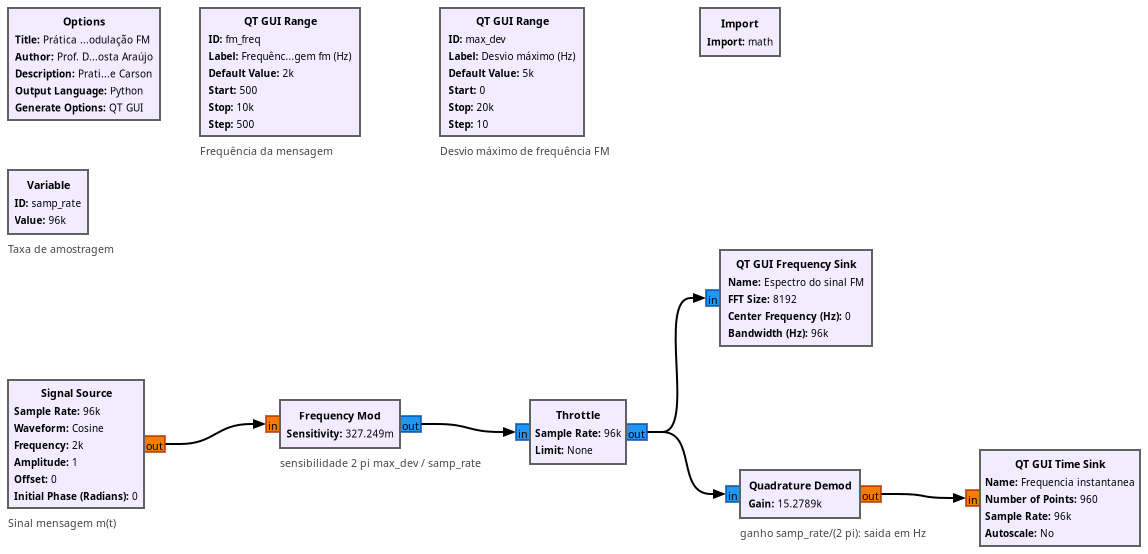
\includegraphics[width=\textwidth]{figuras/flowgraph.png}
  \caption{Flowgraph completo da Prática 05, como aparece no GNU Radio Companion.}
  \label{fig:flowgraph}
\end{figure}

\begin{atencao}[Atenção -- por que \texttt{Frequency Mod} e não \texttt{WBFM Transmit}]
  O bloco \texttt{WBFM Transmit} aplica pré-ênfase, que multiplica o desvio por
  um ganho que cresce com $f_m$: com $\tau=75\,\mu$s e $f_m=2$\,kHz o desvio real
  sai cerca de 50\,\% maior que o ajustado. Além disso, o desvio dele não muda
  com o flowgraph em execução. O \texttt{Frequency Mod} implementa exatamente a
  fase $2\pi k_f\int m(\tau)\,d\tau$, com $k_f = \Delta f$ para $|m(t)|\le 1$, e
  aceita mudança de $\Delta f$ pelo slider durante a execução.
\end{atencao}

% ======================================================
\section{Roteiro de montagem e execução (50 min)}

\subsection*{Parâmetros}

\begin{center}
  \begin{tabular}{l l}
    \toprule
    \texttt{samp\_rate}                      & $96\,000$\,Hz                                                      \\
    \texttt{fm\_freq}, \texttt{QT GUI Range} & $500$ a $10\,000$\,Hz, passo $500$, padrão $2\,000$                \\
    \texttt{max\_dev}, \texttt{QT GUI Range} & $0$ a $20\,000$\,Hz, passo $10$, padrão $5\,000$                   \\
    Signal Source                            & cosseno, amplitude $1$, taxa \texttt{samp\_rate}                   \\
    Frequency Mod, \textit{Sensitivity}      & \texttt{2*math.pi*max\_dev/samp\_rate}                             \\
    Quadrature Demod, \textit{Gain}          & \texttt{samp\_rate/(2*math.pi)}                                    \\
    Frequency Sink                           & FFT $8\,192$, janela \textit{Flat-top}, escala de $-80$ a $10$\,dB \\
    Time Sink                                & $960$ pontos, $100$\,ms, eixo $y$ de $-25\,000$ a $25\,000$        \\
    \bottomrule
  \end{tabular}
\end{center}

\begin{figure}[H]
  \centering
  \begin{subfigure}{0.49\textwidth}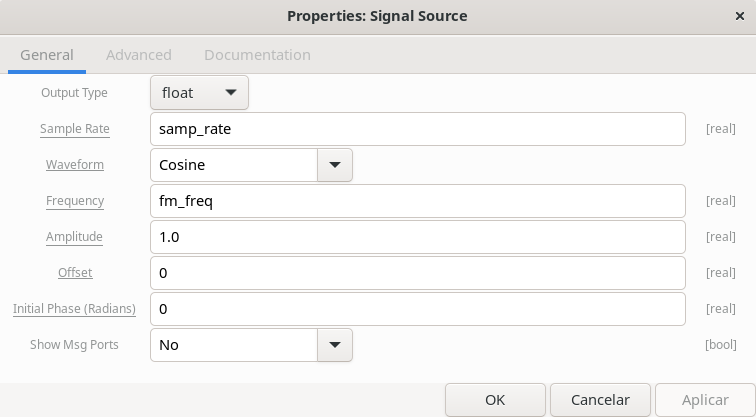
\includegraphics[width=\textwidth]{figuras/bloco_src_mensagem.png}\caption{Signal Source}\end{subfigure}
  \begin{subfigure}{0.49\textwidth}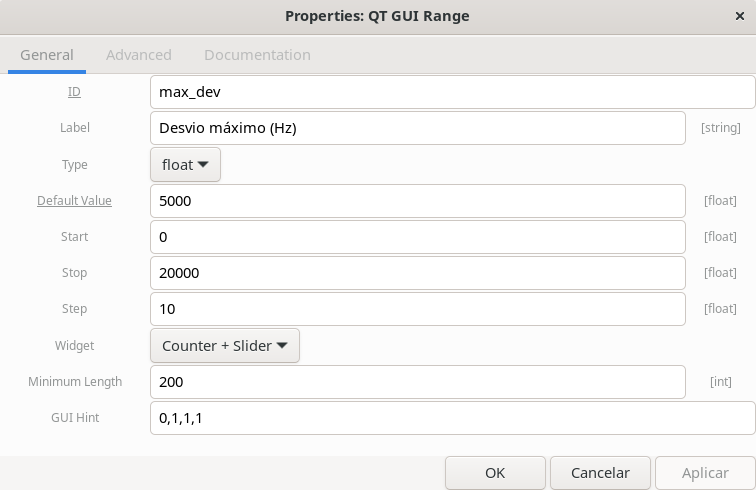
\includegraphics[width=\textwidth]{figuras/bloco_max_dev.png}\caption{QT GUI Range \texttt{max\_dev}}\end{subfigure}\\[4pt]
  \begin{subfigure}{0.49\textwidth}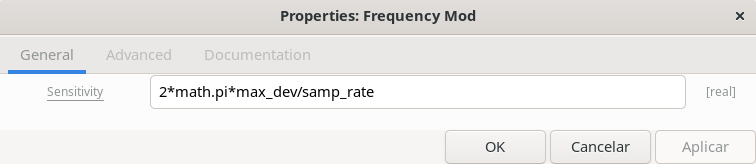
\includegraphics[width=\textwidth]{figuras/bloco_fm_mod.png}\caption{Frequency Mod}\end{subfigure}
  \begin{subfigure}{0.49\textwidth}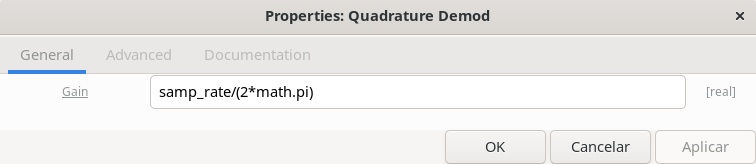
\includegraphics[width=\textwidth]{figuras/bloco_quad_demod.png}\caption{Quadrature Demod}\end{subfigure}
  \caption{Parâmetros dos blocos principais, capturados do GNU Radio Companion.
    O \texttt{QT GUI Range} \texttt{fm\_freq} segue o mesmo modelo do \texttt{max\_dev}.}
  \label{fig:blocos}
\end{figure}

\begin{figure}[H]
  \centering
  \begin{subfigure}{0.49\textwidth}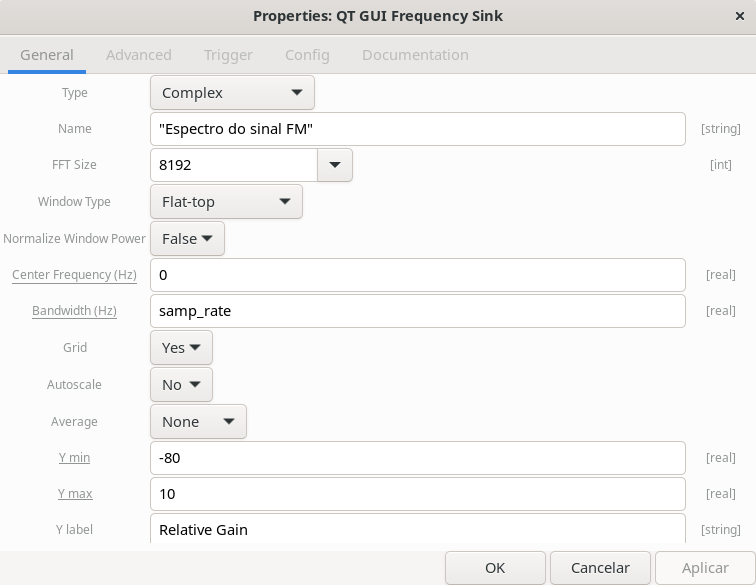
\includegraphics[width=\textwidth]{figuras/bloco_freq_sink_fm.png}\caption{QT GUI Frequency Sink}\end{subfigure}
  \begin{subfigure}{0.49\textwidth}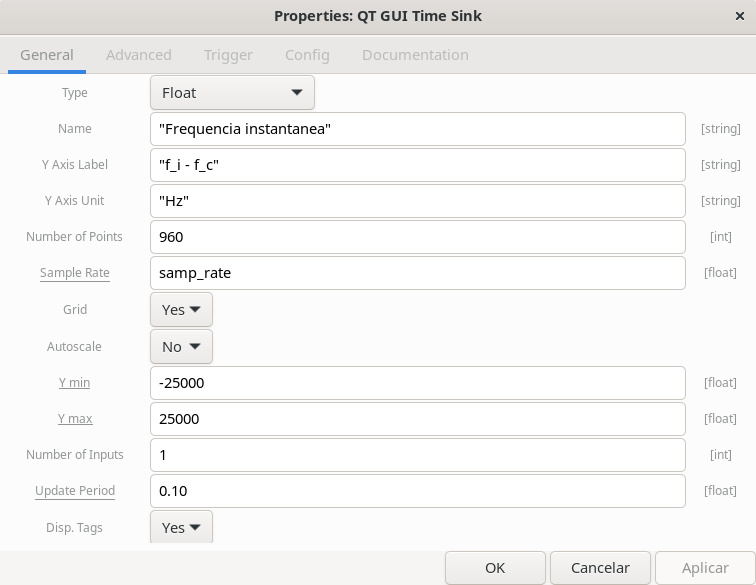
\includegraphics[width=\textwidth]{figuras/bloco_time_sink.png}\caption{QT GUI Time Sink}\end{subfigure}
  \caption{Parâmetros dos instrumentos. No Time Sink, na aba \textit{Trigger},
    use modo \textit{Auto}, nível $0$ e borda positiva para a forma de onda ficar parada.}
  \label{fig:sinks}
\end{figure}

\begin{instrucao}[Leitura dos instrumentos]
  No Frequency Sink, passe o mouse sobre o topo de cada componente para ler a
  frequência e o nível em dB. A janela \textit{Flat-top} foi escolhida porque
  mantém o nível correto mesmo quando a componente cai entre dois pontos da FFT. Arraste com o botão esquerdo para ampliar uma
  região e clique com o botão direito para voltar. No campo numérico do
  \texttt{QT GUI Range} é possível digitar o valor de $\Delta f$ diretamente.
\end{instrucao}

\subsection*{Etapa 1 -- Montagem e níveis das componentes (0--12 min)}

\begin{instrucao}[Níveis em relação à portadora sem modulação]
  \begin{enumerate}[label=\arabic*.]
    \item Monte o flowgraph da Figura~\ref{fig:flowgraph} com os parâmetros acima
          e execute.
    \item Com $f_m = 2\,000$\,Hz, digite $\Delta f = 0$. Leia o nível da única
          componente, em $0$\,Hz. Esse é o nível de referência $L_0$.
    \item Digite $\Delta f = 5\,000$\,Hz, o que dá $\beta=2{,}5$. Leia o nível
          $L_n$ das componentes em $n f_m$ para $n = 0, 1, 2, 3, 4$ e preencha a
          Tabela~\ref{tab:niveis}. Para $n\ge 1$, use a média das leituras em
          $+nf_m$ e $-nf_m$.
  \end{enumerate}
\end{instrucao}

\begin{table}[H]
  \centering
  \begin{tabular}{c c c c c c}
    \toprule
    $n$        & $f$ (kHz)               & $|J_n(2{,}5)|$ & $20\log_{10}|J_n(2{,}5)|$ (dB) &
    $L_n$ (dB) & $L_n - L_0$ medido (dB)                                                         \\
    \midrule
    0          & 0                       & 0,0484         &                                &   & \\
    1          & 2                       & 0,4971         &                                &   & \\
    2          & 4                       & 0,4461         &                                &   & \\
    3          & 6                       & 0,2166         &                                &   & \\
    4          & 8                       & 0,0738         &                                &   & \\
    \bottomrule
  \end{tabular}
  \caption{Níveis das componentes para $f_m = 2$\,kHz e $\Delta f = 5$\,kHz.
    $L_0 = $ \underline{\hspace{2cm}} dB.}
  \label{tab:niveis}
\end{table}

\subsection*{Etapa 2 -- Nulos da portadora (12--20 min)}

\begin{instrucao}[Zeros de $J_0$]
  \begin{enumerate}[label=\arabic*.]
    \item Mantenha $f_m = 2\,000$\,Hz. Partindo de $\Delta f = 4\,500$\,Hz,
          aumente $\Delta f$ em passos de $10$\,Hz até o nível da componente em
          $0$\,Hz passar por um mínimo. Registre esse $\Delta f$ e o nível mínimo
          na Tabela~\ref{tab:nulos}.
    \item Repita partindo de $\Delta f = 10\,700$\,Hz para achar o segundo nulo.
  \end{enumerate}
\end{instrucao}

\begin{table}[H]
  \centering
  \begin{tabular}{c c c c c}
    \toprule
    Zero de $J_0$                & $\Delta f$ teórico (Hz) & $\Delta f$ medido (Hz) &
    Nível mínimo $L_0'-L_0$ (dB) & Erro (\%)                                              \\
    \midrule
    $\beta = 2{,}405$            &                         &                        &   & \\
    $\beta = 5{,}520$            &                         &                        &   & \\
    \bottomrule
  \end{tabular}
  \caption{Nulos da portadora para $f_m = 2$\,kHz. O $\Delta f$ teórico vem da
    equação~\eqref{eq:nulos}.}
  \label{tab:nulos}
\end{table}

\subsection*{Etapa 3 -- Banda medida e regra de Carson (20--36 min)}

\begin{instrucao}[Contagem das componentes acima de $L_0 - 20$\,dB]
  \begin{enumerate}[label=\arabic*.]
    \item Para cada linha da Tabela~\ref{tab:carson}, ajuste $f_m$ e $\Delta f$.
    \item Encontre a maior ordem $n_{\max}$ tal que as componentes em
          $\pm n_{\max} f_m$ ainda estejam com nível maior ou igual a $L_0 - 20$\,dB.
    \item Calcule $B_{\text{med}}$ pela equação~\eqref{eq:bmed}, $B_C$ e o erro
          pela equação~\eqref{eq:carson}.
  \end{enumerate}
\end{instrucao}

\begin{table}[H]
  \centering
  \begin{tabular}{c c c c c c c}
    \toprule
    $f_m$ (Hz)            & $\Delta f$ (Hz) & $\beta$   & $n_{\max}$ &
    $B_{\text{med}}$ (Hz) & $B_C$ (Hz)      & Erro (\%)                       \\
    \midrule
    2\,000                & 1\,000          & 0,5       &            &   &  & \\
    2\,000                & 2\,000          & 1,0       &            &   &  & \\
    2\,000                & 5\,000          & 2,5       &            &   &  & \\
    2\,000                & 10\,000         & 5,0       &            &   &  & \\
    4\,000                & 4\,000          & 1,0       &            &   &  & \\
    4\,000                & 10\,000         & 2,5       &            &   &  & \\
    4\,000                & 20\,000         & 5,0       &            &   &  & \\
    \bottomrule
  \end{tabular}
  \caption{Banda medida pelo critério de $-20$\,dB e regra de Carson.}
  \label{tab:carson}
\end{table}

\subsection*{Etapa 4 -- Discriminador (36--46 min)}

\begin{instrucao}[Frequência instantânea no Time Sink]
  \begin{enumerate}[label=\arabic*.]
    \item Para cada linha da Tabela~\ref{tab:disc}, leia no Time Sink o valor de
          pico $y_{\text{pico}}$ da frequência instantânea, em Hz.
    \item Meça o período $T$ como o intervalo entre duas passagens por zero
          com a mesma inclinação; para mais precisão, meça cinco períodos e divida
          por cinco.
    \item Calcule o erro de $y_{\text{pico}}$ em relação a $\Delta f$ e o índice
          $\beta_{\text{med}} = y_{\text{pico}}/f_m$.
  \end{enumerate}
\end{instrucao}

\begin{table}[H]
  \centering
  \begin{tabular}{c c c c c c c}
    \toprule
    $f_m$ (Hz)      & $\Delta f$ (Hz)  & $y_{\text{pico}}$ (Hz) & Erro (\%) &
    $T$ medido (ms) & $T = 1/f_m$ (ms) & $\beta_{\text{med}}$                        \\
    \midrule
    2\,000          & 1\,000           &                        &           &   &  & \\
    2\,000          & 5\,000           &                        &           &   &  & \\
    2\,000          & 10\,000          &                        &           &   &  & \\
    4\,000          & 10\,000          &                        &           &   &  & \\
    \bottomrule
  \end{tabular}
  \caption{Medições na saída do \texttt{Quadrature Demod}.}
  \label{tab:disc}
\end{table}

\subsection*{Síntese (46--50 min)}

Confira se todas as tabelas estão preenchidas, com unidades e erros calculados.

\begin{atencao}[Atenção -- escopo desta prática]
  Esta prática trata da modulação e da demodulação FM sem ruído. Os detectores de
  inclinação e o discriminador balanceado são tratados na Prática 06.
\end{atencao}

% ======================================================
\section{Perguntas para o relatório}

Todas as respostas devem ser numéricas, com as contas mostradas.

\begin{enumerate}[label=\textbf{Q\arabic*.}, leftmargin=*]

  \item Na Tabela~\ref{tab:niveis}, qual é a maior diferença, em dB, entre o
        nível medido e $20\log_{10}|J_n(2{,}5)|$? Converta essa diferença $d$ para
        erro de amplitude, $100\,(10^{d/20}-1)\,\%$.

  \item Na Tabela~\ref{tab:nulos}, calcule o erro percentual de cada nulo e a
        razão entre o segundo e o primeiro $\Delta f$ medidos. Compare essa razão
        com $5{,}520/2{,}405$.

  \item Na Tabela~\ref{tab:carson}, para quais valores de $\beta$ o erro de
        Carson é nulo, e quanto vale o erro para $\beta=0{,}5$ e $\beta=2{,}5$?
        Usando a Tabela~\ref{tab:bessel}, calcule a fração da potência dentro de
        $B_{\text{med}}$, $J_0^2+2\sum_{n=1}^{n_{\max}}J_n^2$, para $\beta = 0{,}5$,
        $2{,}5$ e $5$.

  \item Para $\beta = 2{,}5$, $B_C$ é maior que $B_{\text{med}}$. Quantas
        componentes de frequência existem entre $B_{\text{med}}/2$ e $B_C/2$, e
        quanto a potência dentro de $B_C$ difere da potência dentro de
        $B_{\text{med}}$?

  \item Com $\Delta f = 10$\,kHz fixo, $f_m$ passou de 2 para 4\,kHz. Calcule a
        razão entre as bandas medidas e a razão entre as bandas de Carson. Faça o
        mesmo com $\beta = 5$ fixo, entre $f_m = 2$ e $4$\,kHz.

  \item Na Tabela~\ref{tab:disc}, qual é o maior erro de $y_{\text{pico}}$ e de
        $T$? Compare $\beta_{\text{med}}$ com $\Delta f/f_m$ em cada linha.

\end{enumerate}

% ======================================================
\appendix
\section{Valores de $|J_n(\beta)|$}

\begin{table}[H]
  \centering
  \begin{tabular}{c c c c c c c c c c}
    \toprule
    $\beta$ & $n=0$  & $1$    & $2$    & $3$    & $4$    & $5$    & $6$    & $7$    & $8$    \\
    \midrule
    0,5     & 0,9385 & 0,2423 & 0,0306 & 0,0026 & 0,0002 & 0,0000 & 0,0000 & 0,0000 & 0,0000 \\
    1,0     & 0,7652 & 0,4401 & 0,1149 & 0,0196 & 0,0025 & 0,0002 & 0,0000 & 0,0000 & 0,0000 \\
    2,5     & 0,0484 & 0,4971 & 0,4461 & 0,2166 & 0,0738 & 0,0195 & 0,0042 & 0,0008 & 0,0001 \\
    5,0     & 0,1776 & 0,3276 & 0,0466 & 0,3648 & 0,3912 & 0,2611 & 0,1310 & 0,0534 & 0,0184 \\
    \bottomrule
  \end{tabular}
  \caption{Valores de $|J_n(\beta)|$ usados nas Tabelas~\ref{tab:niveis}
    e~\ref{tab:carson}. O critério de $-20$\,dB corresponde a $|J_n|\ge 0{,}1$.}
  \label{tab:bessel}
\end{table}

% ======================================================
\section*{Entregáveis}

Relatório em PDF contendo:
\begin{itemize}
  \item As Tabelas~\ref{tab:niveis} a~\ref{tab:disc} preenchidas, com $L_0$.
  \item Captura do espectro para $f_m = 2$\,kHz com $\Delta f = 0$,
        $5\,000$\,Hz e no primeiro nulo.
  \item Captura do Time Sink para $f_m = 2$\,kHz e $\Delta f = 5\,000$\,Hz.
  \item Respostas às perguntas Q1 a Q6.
\end{itemize}

\end{document}
